%% DTK Domain Model

\documentclass[letterpaper,12pt]{article}
\usepackage[top=1.0in,bottom=1.0in,left=1.25in,right=1.25in]{geometry}
\usepackage{appendix}
\usepackage{verbatim}
\usepackage{amssymb}
\usepackage{graphicx}
\usepackage{longtable}
\usepackage{amsfonts}
\usepackage{amsmath}
\usepackage{algpseudocode} 
\usepackage[usenames]{color}
\usepackage[
  naturalnames = true, 
  colorlinks = true, 
  linkcolor = black,
  anchorcolor = black,
  citecolor = black,
  menucolor = black,
  urlcolor = blue
]{hyperref}
\usepackage{listings}
\usepackage{textcomp}

%%---------------------------------------------------------------------------%%
\author{
  Stuart R. Slattery\\
  Department of Engineering Physics\\
  University of Wisconsin - Madison\\
  1500 Engineering Dr.\\
  Madison, WI 53716 \\
  \href{mailto:sslattery@wisc.edu}{\texttt{sslattery@wisc.edu}}
}

\date{\today}
\title{A Rendezvous-Based Domain Model for \\ Data Transfer}
\begin{document}
\maketitle

\newpage

%%---------------------------------------------------------------------------%%
\begin{abstract}
  In many physics applications, the concept of mesh is used to
  subdivide physical domain into a discrete representation to
  facilitate the solution of the model problems that describe
  it. Additionally, the concept of the field is used to apply degrees
  of freedom to the mesh as an additional means of
  discretization. With the increased development efforts in
  multiphysics simulation, adaptive simulations, and other multiple
  mesh problems, transferring fields and other data between meshes is
  a common operation. This document describes a domain model for mesh,
  fields, and data transfer based on the concept of geometric
  rendezvous and its implementation within the Data Transfer Kit
  software package.
\end{abstract}

\newpage
\newpage

%%---------------------------------------------------------------------------%%
\tableofcontents
\clearpage
\listoffigures
\clearpage
\listoftables
\newpage
\newpage

%%---------------------------------------------------------------------------%%
\section{Introduction}\label{sec:intro}
In many physics applications, it is often desired to transfer fields
(i.e. degrees of freedom or other data) between meshes that may or may
not conform in physical space. In addition, for massively parallel
simulations, it is typical that meshes not only do not conform
spatially, but also that their parallel decompositions do not
correlate and are independent of one another due to physics-based
partitioning requirements. As an example, this situation can occur in
multiphysics simulations where physics fields provide feedback between
solution iterations or adaptive mesh simulations where fields must be
moved between meshes after refining and coarsening. It is therefore
desirable to have a set of tools to relate two meshes of arbitrary
parallel decomposition such that fields and other data can be
transferred between them.

The Data Transfer Kit (DTK) is a software component designed to
provide parallel services for mesh repartitioning, mesh searching, and
data transfer based on the concept of the rendezvous decomposition
\cite{Plimpton_2004}. To achieve a component design for use with
arbitrary physics codes, general concepts of mesh and fields are
employed to provide access to these services. This document will
outline the concepts of parallel communicators, mesh, fields, data
transfer, and the rendezvous decomposition and how they are modeled
within the design of DTK.

\clearpage

%%---------------------------------------------------------------------------%%
\section{Communicators}\label{sec:communicators}
A communicator is a concept that encapsulates ownership of operations
in a parallel computation. A parallel communicator in the context of
DTK can be taken as a direct reference to a Message Passing Interface
(MPI) communicator \cite{MPI_1994}. A single communicator has set of
process space over which it may perform operations. Multiple
communicators may exist in a single process space and own the same
processes. 

Based on this, we can consider two likely operations which will we
want to perform. A union operation will compute the union in process
space of all communicators involved. Figure~\ref{fig:comm_union}
provides an example of a union operation. An intersection operation
will compute the intersection in process space of all communicators
involved. Figure~\ref{fig:comm_intersection} provides an example of an
intersection operation.


\clearpage

%%---------------------------------------------------------------------------%%
\section{Mesh}\label{sec:mesh}
In order to access DTK services, a subset of the information regarding
the mesh is required. This subset consists of nodes and their
coordinates, and elements and the nodes that construct them. This
subset has been demonstrated as sufficient for applying data transfer
algorithms \cite{Stewart_2004} and can be formulated in such a way
that algorithms can be generated that are data structure netural
\cite{Chand_2008}. In addition, for meshes that contain multiple
element topologies, the concept of mesh blocked by element topology is
utilized. For meshes decomposed in parallel, the term global will be
used to refer to concepts that apply across the entire parallel domain
while the term local will be used to refer to concepts that only exist
in the domain of a single parallel process. 

\subsection{Mesh Nodes}\label{subsec:nodes}
Nodes are the lowest level geometric component of the mesh. All nodes
have a globally unique ordinal serving as an identification number for
the node in global operations. A node can have 1, 2, or 3 dimensions
but all nodes in a mesh must have the same dimension. To specify its
geometric position, each node has Cartesian (x,y,z) coordinates. A
node must provide only the coordinates for the specified node
dimension, no more or no less (e.g. a 2 dimensional node must provide
x and y coordinates but not a z coordinate). A node may be repeated
any number of times across the parallel domain with unlimited local
and global instances. However, every node with the same globally
unique ordinal must have the same coordinates. As an example, consider
Figure~\ref{fig:mesh_nodes} depicting a series of nodes contained in
a mesh. Each node provides a globally unique ordinal and set of 3
dimensional coordinates.

\begin{figure}[htpb!]
  \centering
  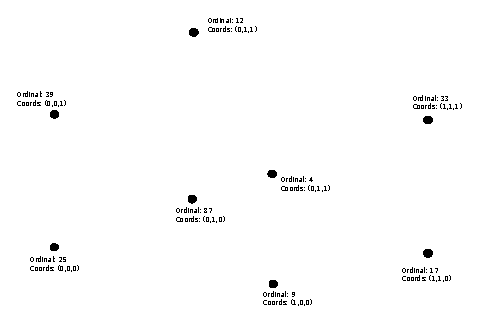
\includegraphics[width=5in]{hex_nodes.eps}
  \caption{\sl Basic node description for a mesh. Each node is
    required to have a unique global ordinal, a specified
    dimensionality, and Cartesian coordinates corresponding to that
    dimensonality. The nodes in this example are 3 dimensional.}
  \label{fig:mesh_nodes}
\end{figure}

\subsection{Mesh Elements}\label{subsec:elements}
Elements are the second level of abstraction in the mesh description
above nodes. All elements have a globally unique ordinal serving as an
identification number for the element in global operations. This
globally unique ordinal can be the same as a globally unique ordinal
for a node in the mesh as DTK distinguishes between nodes and
elements. An element has a topology defining its physical structure
(e.g. tetrahedron, hexahedron, etc.) and a number of nodes needed to
generate that topology. Elements are constructed from nodes via a
connectivity list. The connectivity list for a particular element will
contain the unique node global ordinals that construct it. An element
may be repeated any number of times across the parallel domain
(i.e. it may have unlimited local instances), however, every globally
unique ordinal must have the same connectivity list associated with
it. For consistency, DTK uses the MoaB Canonical Numbering (MBCN)
scheme as a canonical ordering scheme \cite{Tautges_2009}. Each
element in a client mesh can be described with a connectivity list
using any canonical scheme of choice, however, the relationship
between this canonical numbering scheme and the DTK canonical
numbering scheme must be made available. Each element topology is then
also described by a permutation list. A permutation list specifies the
variation in ordering between the DTK canonical numbering scheme and
the client canonical numbering scheme. For elements that have a higher
order basis (e.g. quadratic), DTK resolves these as higher order nodes
via the MBCN system. See Appendix~\ref{apdx:cell_topo} for canonical
element topologies.

Consider the continuation of our example in
Figure~\ref{fig:mesh_element} showing a linear hexahedron element
generated from the nodes in Figure~\ref{fig:mesh_nodes}. The element
has been given a unique global ordinal and the connectivity and
permuation lists have been specified. The connectivity list specifies
an element construction from counter-clockwise movement around the
bottom face and then counter-clockwise movement around the top face
that is native to the client. The MBCN canonical ordering for linear
hexahedrons is given at the nodes. Note that this ordering instead
uses clockwise rotation around the bottom and top faces to construct
the element. This difference in ordering is specified by the given
permutation list.

\begin{figure}[htpb!]
  \centering
  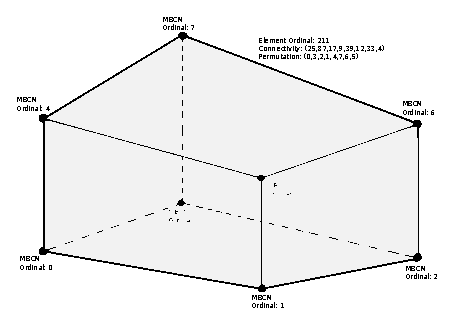
\includegraphics[width=5in]{hex_element.eps}
  \caption{\sl Basic element description for a mesh. Each element is
    required to have a unique global ordinal, and a specified
    connectivity and permuation list. The MBCN canonical ordinals used
    by DTK are specified at the nodes.}
  \label{fig:mesh_element}
\end{figure}

\subsection{Mesh Blocks}\label{subsec:blocks}
At the highest level of abstraction, the mesh is composed of mesh
blocks. These blocks contain elements of the same topology and number
of nodes. All elements in a block must have the same topology and
number of nodes. A mesh may contain as many blocks as
desired. Multiple blocks with the same mesh topology may exist. Nodes
may be repeated in different mesh blocks provided that they maintain
the same unique global ordinal and coordinates. Elements may be
repeated in different mesh blocks provided that they maintin the same
unique global ordinal and connectivity list. Multiple mesh blocks may
exist in the same spatial region as they are merely a means of
subdividing the mesh into groups of elements based on their
topology. This behavior will be the common when hybrid meshes are
involved (e.g. a mesh that contains hexahedrons and
tetrahedrons). Mesh blocks may be either structured or unstructured.

As an example, consider the 2 dimensional hybrid mesh presented in
Figure~\ref{fig:hybrid_mesh}. This mesh contains both quadrilateral
(blue) and triangle (red) elements that share connecting nodes. In
this case, all quadrilaterals should be specified in a single mesh
block and all triangles specified in another mesh block. The nodes
shared by these two mesh blocks may be repeated in either block.

\begin{figure}[htpb!]
  \centering
  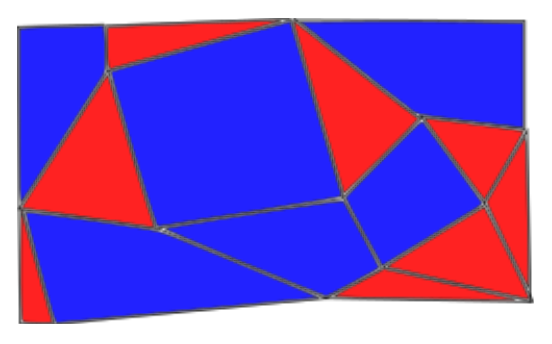
\includegraphics[width=5in]{hybrid_mesh.eps}
  \caption{\sl Hybrid mesh example. Quadrilaterals (blue) must be
    specified in a different mesh block than the triangles (red). Both
    blocks can share mesh nodes.}
  \label{fig:hybrid_mesh}
\end{figure}

\subsection{Parallel Decomposition}\label{subsec:mesh_decomp}
Mesh blocks and the elements and nodes they contain may be partitioned
in any fashion provided that all nodes, elements, and blocks of a mesh
description exist in a communication space operated by the same
parallel communicator. Different blocks in a single mesh description
may not have different communicators. Each mesh description may have
its own communicator. Global knowledge of the parallel decomposition
of a given mesh description is not required. Only local mesh data
access along with the proper communicator is required.

\clearpage

%%---------------------------------------------------------------------------%%
\section{Geometric Rendezvous}\label{sec:rendezvous}
Relating two non-conformal meshes will ultimately require some type of
evaluation algorithm to apply the data from one mesh to another. To
achieve this, the target objects to which this data will be applied
must be located within the the source geometry. In a serial
formulation, efficient search structures that offer logarithmic
asymptotic time complexity are available to perform this
operation. However, in a parallel formulation, if these two meshes are
arbitrarily decomposed, then a certain degree of communication will be
required as well as geometric alignment is not likely.

A geometry that is associated with the data that will be transferred
will be referred to as the source geometry while the the geometry that
will be receiving the data will be referred to as the target geometry.

\subsection{The Rendezvous Algorithm}\label{subsec:rendezvous_alg}
The geometric rendezvous concept uses a global formulation for the
data transfer while maintaining a local formulation for the geometric
search operations. In DTK, the following algorithm generated by
Plimpton et. al. \cite{Plimpton_2004} generates the rendezvous
decomposition through global operations in order to achieve a local
framework for geometric operations. 

\begin{enumerate}
\item Compute a box that bounds the source and target geometry
  intersection.
\item Create a rendezvous decomposition by performing recursive
  coordinate bisectioning on the source geometry.
\item Send source geometry from the source decomposition to rendezvous
  decomposition.
\item Clone source geometry components which overlap into nearby
  recursive coordinate bisectioning sub-domains.
\item Build a kD-tree with the local mesh in each rendezvous
  partition.
\end{enumerate}

This algorithm is elaborated in more detail in the following
paragraphs.

\paragraph{Step 1: Bounding box construction.}
To begin, a global bounding box for the source and target geometries
is constructed using their nodal data. These two bounding boxes are
then intersected to produce the bounding box around the intersection
of the two geometries. Those source or target nodes that are not
inside this intersection bounding box are not considered for
evaluation. This step is motivated by the fact that for many classes
of data transfer problems, such as 2D surface transfer in a full 3D
problem, only a small subset of the source and target geometries will
be used. This will reduce the number of search operations and
communication operations.

\paragraph{Step 2: Rendezvous decomposition generation.}
Recursive coordinate bisectioning (RCB) is used the create a new
decomposition with the source mesh nodes \cite{Berger_1987}.

\paragraph{Step 3: Send source elements to rendezvous decomposition.}
The RCB decomposition is generated only from source node
information. The element information must be sent to the rendezvous
decomposition for the point location process. 

\paragraph{Step 4: Clone source elements that overlap RCB
  sub-domains.}  Because RCB was performed using source nodal data,
there will be source elements that span the boundary between two or
more RCB sub-domains. When this occurs, the source elements will be
repeated in each RCB sub-domain in which their connectivity nodes
exist. 

\paragraph{Step 5: Build a kD-tree with the local mesh in each rendezvous
  partition.}  On each rendezvous process, the local mesh is will be
searched with the local target nodes. An adaptive kD-tree is generated
using the local mesh for a fast proximity search of the domain that
computes a subset of the local mesh that resides near the node
\cite{Bentley_1975}. This subset is then searched with a more
expensive point-in-element operation that transforms the node into the
reference frame of each element in the subset and uses a Newton
iteration strategy to determine if the node is contained within.

\subsection{The Rendezvous Decomposition}\label{subsec:rendezvous_decomp}
Using the above algorithm, a secondary decomposition of a subset of
the source mesh is generated forming the rendezvous decomposition. The
rendezvous decomposition is encapsulated as a separate entity from the
original geometric description of the domain. It can be viewed most
formally as a copy of the source mesh subset that intersects the
target geometry. This copy has been repartitioned in a way that
fundamental geometric search operations are local and proceed globally
in a load balanced fashion.

The rendezvous decomposition has several properties. It is defined
over a communicator that encapsulates the union of the communication
spaces owned by the source and target geometries. It is defined inside
of a global, axis-aligned bounding box that bounds the intersection of
the source and target geometries. The decomposition is of the same
dimension as the source and target geometries. A rendezvous
decomposition cannot be generated with source and target geometries of
different dimensions (e.g. a 3 dimensional source geometry and a 2
dimensional target geometry cannot be used to generate a rendezvous
decomposition). Global recursive coordinate bisectioning parameters
are maintained for global partitioning information. A local kD-tree is
formed over the local mesh. In this way, mesh searches on the global
level use the RCB partitioning information and mesh searches on the
local level use the kD-tree with both operations exhibiting
O(n*log(n)) asymptotic time and space complexity for generating and
searching the appropriate data structures.

\clearpage

%%---------------------------------------------------------------------------%%
\section{Fields}\label{sec:field}

\subsection{Fields of Multiple Dimensions}\label{subsec:field_dim}

\subsection{Field Evaluations}\label{subsec:eval}

\subsection{Basic Field Operations}

\clearpage

%%---------------------------------------------------------------------------%%
\section{Mesh/Field Mapping}\label{sec:map}

\begin{enumerate}
\item Find which rendezvous sub-domain each target geometry component
  is inside of.
\item Send target geometry from target decomposition to rendezvous
  decomposition.
\item Find which target geometry component is inside which source
  geometry component.
\item Send source/target pairings from rendezvous decomposition to
  source decomposition.
\end{enumerate}

\paragraph{Step 1: Find rendezvous subdomain for target nodes.}
On each target process, the RCB decomposition is searched to find the
destination process for the target node in the rendezvous
decomposition.

\paragraph{Step 2: Send target nodes to rendezvous decomposition.}
Each target node is moved to the appropriate RCB sub-domain for the
point location step.

\paragraph{Step 3: Find source elements in which target nodes reside.}
We now have source element information and target node information in
the rendezvous decomposition. On each rendezvous process, the local
mesh is searched with the local target nodes using the adaptive
kD-tree and underlying point-in-element functionality.

\paragraph{Step 4: Send element/node pairs back to original
  decompositions.}  The source element/target node pairs are the map
in this case and they will be used to drive the evaluation
routines. These pairings must be communicated from the rendezvous
decomposition back to the source/target decompositions to complete the
mapping.

\clearpage

%%---------------------------------------------------------------------------%%
\section{Transfer Operations}\label{sec:transfer}

\clearpage

%%---------------------------------------------------------------------------%%
\section{Conclusion}\label{sec:conc}

\clearpage

%%---------------------------------------------------------------------------%%
\appendix
\section{DTK Element Topologies}\label{apdx:cell_topo}

%%---------------------------------------------------------------------------%%
\pagebreak
\bibliographystyle{ieeetr}
\bibliography{references}
\end{document}


